\documentclass{anstrans}
%%%%%%%%%%%%%%%%%%%%%%%%%%%%%%%%%%%
\title{Comparing HALEU Demand Among Advanced Reactor Fuel Cycle Transitions}
\author{Amanda M. Bachmann, Kathryn D. Huff}

\institute{
Dept. of Nuclear, Plasma and Radiological Engineering, University of Illinois at Urbana-Champaign \\
amandab7@illinois.edu
}

%%%% packages and definitions (optional)
\usepackage{graphicx} % allows inclusion of graphics
\graphicspath{{./figures/}}
\usepackage{float}
\usepackage{booktabs} % nice rules (thick lines) for tables
\usepackage{microtype} % improves typography for PDF
\usepackage{xspace}
\usepackage{tabularx}
\usepackage{amsmath}
\usepackage{subcaption}
\usepackage{enumitem}
\usepackage{placeins}
\usepackage{tikz}
\usepackage{hyperref}

\usepackage{tikz}
\usetikzlibrary{shapes.geometric, arrows}
\usetikzlibrary{positioning, arrows, decorations, shapes}

\tikzstyle{facility} = [rectangle, rounded corners, minimum width=2cm, minimum height=0.75cm,text centered, draw=black, fill=blue!30]
\tikzstyle{transition} = [rectangle, rounded corners, minimum width=2cm, minimum height=0.75cm,text centered, draw=black, fill=red!30]
\tikzstyle{arrow} = [thick,->,>=stealth]

\usepackage[acronym,toc]{glossaries}
\include{acros}
\makeglossaries
\newcommand{\Cyclus}{\textsc{Cyclus}\xspace} %
\newcommand{\Cycamore}{\textsc{Cycamore}\xspace} %

\begin{document}

%%%%%%%%%%%%%%%%%%%%%%%%%%%%%%%%%%%%%%%%%%%%%%%%%%%%%%%%%%%%%%%%%%%%%%%%%%%%%%%%
\section{Introduction}
The \gls{LWR} that are currently employed for commercial power in the 
United States all use similar fuel forms at \gls{LEU} enrichment levels 
less than 5\%. New reactor designs, such as the \gls{USNC} \gls{MMR} will 
use \gls{LEU} fuel enriched between 5-20\%, often referred to as \gls{HALEU}.

To meet the demand for \gls{HALEU} fuel for advanced reactors, the U.S. 
\gls{DOE} has proposed two methods to achieve fuel at the 
required enrichment level: recovery and downblending of \gls{HEU} fuel 
from EBR-II and other \gls{DOE} owned \gls{HEU} fuel or enriching natural 
uranium to the desired level \cite{griffith_overview_2020}. Each of these 
methods to produce \gls{HALEU} fuel has its limitations. Downblending
\gls{HEU} fuel is limited by the existing physical supply of \gls{HEU}
fuel and downblending capacity. Enrichment of natural uranium is limited by
the centrifuge capacity in terms of \gls{SWU} and throughput.

This works quantifies the resource requirements for multiple transition 
scenarios. Resource requirements include enriched fuel amount at each 
enrichment level, \gls{HEU} amount, natural uranium amount, and \gls{SWU} 
capacity required to meet \gls{HALEU} demand for each transition scenario. 
These quantities will inform material requirements and possible methods to 
meet fuel demand for each transition scenario. 

%%%%%%%%%%%%%%%%%%%%%%%%%%%%%%%%%%%%%%%%%%%%%%%%%%%%%%%%%%%%%%%%%%%%%%%%%%%%%%%%
%\input{motivation}

%%%%%%%%%%%%%%%%%%%%%%%%%%%%%%%%%%%%%%%%%%%%%%%%%%%%%%%%%%%%%%%%%%%%%%%%%%%%%%%%
%\input{background}

%%%%%%%%%%%%%%%%%%%%%%%%%%%%%%%%%%%%%%%%%%%%%%%%%%%%%%%%%%%%%%%%%%%%%%%%%%%%%%%%
\section{Methodology}

Each fuel cycle scenario is simulated using \Cyclus, an 
agent-based fuel cycle simulator \cite{huff_fundamental_2016}. 
The agent-based architecture of \Cyclus allows for the simulation to treat
each facility discretely, including their deployment and 
decommissioning \cite{huff_fundamental_2016}. The \Cyclus 
Additional Modules Repository (the \Cycamore library) provides 
the archetypes for each of the facility agents deployed in the simulation.

The first scenario only simulates the current fleet of U.S. reactors. This 
simulation begins in January 1965 and lasts through December 2090 (125 
years in total) with one month timesteps. The \gls{IAEA} \gls{PRIS} 
database \cite{noauthor_power_1989} 2020 
Year-end Reactor Status Report provided information about each reactor.
This database provides reactor type, rated power level, start-up, and 
shutdown dates for each of the commercial reactors in the U.S. reactor 
fleet (as of December 2020). The simulations assume 
the \gls{LWR}s operate for 60 years after their
initial start date if they have not already been shut down. Only reactors
with a power level above 400 MWe were 
used in the simulation to avoid including prototype and research reactors 
present in the database. Generic reactor core masses were obtained from 
\cite{todreas_nuclear_2012} and \cite{cacuci_handbook_2010}. 

As Figure \ref{fig:fuel_cycle} shows, other fuel cycle facilities deployed 
include: a uranium mine (to 
represent the Cameco Smith Ranch-Highland Mine), a uranium mill (to 
represent White Mesa Uranium Mill), a conversion facility (to represent 
the Honeywell Uranium Conversion Facility), an enrichment plant (to represent 
the Portsmouth Gaseous Diffusion Plant), a fuel fabrication facility (to 
represent the Westinghouse Fuel Fabrication Facility), and various waste and 
spent fuel storage and disposal facilities (to represent Yucca Mountain). 
While there
are other fuel cycle facilities in the actual U.S. fuel cycle, this 
modeling provides a concise total of the resources required 
by each non-reactor step in the nuclear fuel cycle and simplifies the 
facilities that are not expected to be deployed or decommissioned often 
during the specified time frame. Most of these facilities do not have 
any limits on their production throughputs, except the fuel fabrication 
plant, which has a front end storage limit of 1 million kg of enriched 
uranium. 

\begin{figure}[ht]
    \centering
    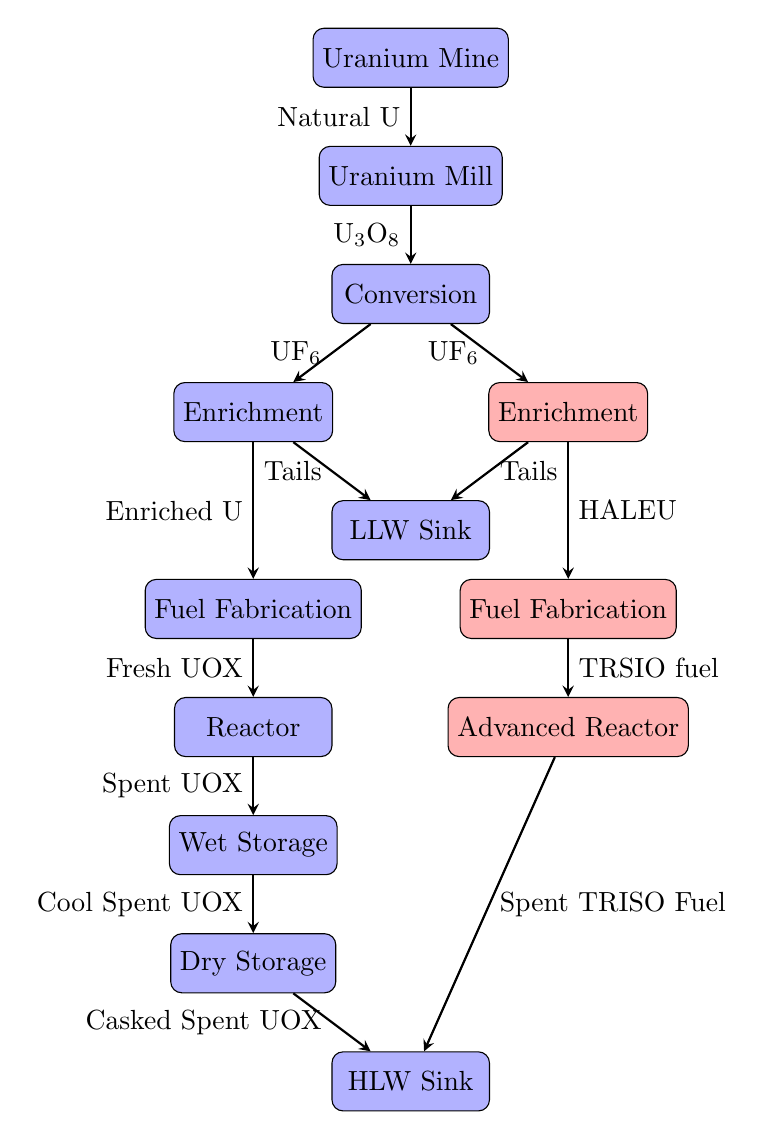
\begin{tikzpicture}[node distance=1.5cm]
        \node (mine) [facility] {Uranium Mine};
        \node (mill) [facility, below of=mine] {Uranium Mill};
        \node (conversion) [facility, below of=mill] {Conversion};
        \node (enrichment) [facility, below of=conversion, xshift=-2cm]{Enrichment};
        \node (enrichment2) [transition, below of=conversion, xshift=2cm]{Enrichment};
        \node (fabrication2) [transition, below of=enrichment2,yshift=-1cm]{Fuel Fabrication};
        \node (fabrication) [facility, below of=enrichment, yshift=-1cm]{Fuel Fabrication};
        \node (reactor) [facility, below of=fabrication]{Reactor};
        \node (adv_reactor) [transition, below of=fabrication2]{Advanced Reactor};
        \node (wetstorage) [facility, below of=reactor]{Wet Storage};
        \node (drystorage) [facility, below of=wetstorage]{Dry Storage};
        \node (sinkhlw) [facility, below of=drystorage, xshift=2cm]{HLW Sink};
        \node (sinkllw) [facility, below of=enrichment, xshift=2cm]{LLW Sink};

        \draw [arrow] (mine) -- node[anchor=east]{Natural U} (mill); 
        \draw [arrow] (mill) -- node[anchor=east]{U$_3$O$_8$}(conversion); 
        \draw [arrow] (conversion) -- node[anchor=east]{UF$_6$}(enrichment);
        \draw [arrow] (enrichment) -- node[anchor=east]{Enriched U}(fabrication);
        \draw [arrow] (conversion) -- node[anchor=east]{UF$_6$}(enrichment2);
        \draw [arrow] (enrichment2) -- node[anchor=west]{HALEU}(fabrication2);
        \draw [arrow] (enrichment) -- node[anchor=east]{Tails}(sinkllw);
        \draw [arrow] (enrichment2) -- node[anchor=west]{Tails}(sinkllw);
        \draw [arrow] (fabrication) -- node[anchor=east]{Fresh UOX}(reactor);
        \draw [arrow] (fabrication2) -- node[anchor=west]{TRSIO fuel}(adv_reactor);
        \draw [arrow] (reactor) -- node[anchor=east]{Spent UOX}(wetstorage);
        \draw [arrow] (wetstorage) -- node[anchor=east]{Cool Spent UOX}(drystorage);
        \draw [arrow] (drystorage) -- node[anchor=east]{Casked Spent UOX}(sinkhlw);
        \draw [arrow] (adv_reactor) -- node[anchor=west]{Spent TRISO Fuel}(sinkhlw);

        \end{tikzpicture}
    \caption{Fuel cycle facilities and material flow between facilities. Facilities in 
    red are deployed in the transition scenarios.}
    \label{fig:fuel_cycle}
\end{figure}

There are multiple reactor agents in each of the scenarios, one agent for 
each reactor, which are condensed to one facility in Figure 
\ref{fig:fuel_cycle}. The facilities shown in red are used only in the 
transition scenarios to provide a separate material stream. 

Other fuel cycle scenarios simulated include the transition to a future with 
substantial \gls{HALEU} 
reactor deployment under two assumptions about growth in nuclear energy 
demand: one simulation assuming no growth and the other assuming 1\% annual 
growth. The different scenarios in this work are summarized in Table 
\ref{tab:scenarios}.  
The transition to the new reactor type starts in 2025. 
These scenarios used the same  
non-reactor facilities as in the simulation of the current 
U.S. fuel cycle. \gls{HALEU} fuel reactors 
considered in this work include the \gls{USNC} \gls{MMR} \textsuperscript{TM}
\cite{mitchell_usnc_2020} and the X-Energy Xe-100 \textsuperscript{TM} 
Reactor \cite{harlan_x-energy_2018}\cite{hussain_advances_2018}. Both of 
these reactors are designed 
to use \gls{HALEU} fuel in the form of \gls{TRISO} fuel particles. Table 
\ref{tab:reactor_summary} summarizes the key design characteristics of these 
two reactors.

\begin{table}[ht]
    \caption{Fuel cycle scenarios}
    \label{tab:scenarios}
    \begin{tabular}{p{2cm}p{3cm}p{2.5cm}}
        \hline
        Scenario No. & Advanced Reactor & Demand Growth \\\hline
        1 & None & N/A \\
        2 & \gls{USNC} \gls{MMR} & No growth \\
        3 & X-energy Xe-100 & No growth \\
        4 & \gls{USNC} \gls{MMR} & 1\% growth\\
        5 & X-energy Xe-100 & 1\% growth\\
        \hline
    \end{tabular}
\end{table}

\begin{table}[ht]
    \caption{Mico-reactor design specifications}
    \label{tab:reactor_summary}
    \begin{tabular}{l p{2.5cm}p{2.25cm}p{2.4cm}}
        \hline
        Design Criteria & \gls{USNC} \gls{MMR}\textsuperscript{TM} & 
            X-Energy Xe-100\textsuperscript{TM} \\\hline
        Reactor type & Modular HTGR & Modular HTGR \\
        Power Output (MWth) & 15 & 200 \\
        Enrichment (\% $^{235}U$) & 13 & 15.5 \\
        Cycle Length (years) & 20 & online refuel\\
        Fuel form & \gls{TRISO} compacts & \gls{TRISO} pebbles\\
        Reactor Lifetime & 20 years & 60 years \\
        Coolant & He & He \\
        \hline
    \end{tabular}
\end{table}
    
We selected these two reactors because they have a high 
likelihood of being deployed and because published information is 
available about their designs. Comparing the transitional \gls{HALEU} 
demands of these reactors will also inform the fuel cycle support 
implications of deploying reactors with long cycle 
times versus those utilizing online refueling. 

Each of the transition scenarios have been simulated using a single type of 
advanced reactor, resulting in four additional fuel cycle scenarios and five 
scenarios in total. Each of the scenarios will be analyzed using Cymetric
\cite{scopatz_cymetric_2015} to determine the resource requirements of the 
scenario. 



%%%%%%%%%%%%%%%%%%%%%%%%%%%%%%%%%%%%%%%%%%%%%%%%%%%%%%%%%%%%%%%%%%%%%%%%%%%%%%%%
\section{Results}

The results include the time-dependent resources required 
for each of the transition scenarios described. Resource requirements
of interest include the annual mass of enriched uranium required by 
the scenario (at each enrichment level), the amount of 
\gls{SWU} required to meet the annual product requirement, the amount 
of \gls{HEU} required for downblending to meet annual fuel requirements, 
and the rate of reactor deployment to meet the 
electricity demand of the scenario. Each of these resources will help
to determine an optimal way to meet \gls{HALEU} fuel demand for each 
scenario. 



%%%%%%%%%%%%%%%%%%%%%%%%%%%%%%%%%%%%%%%%%%%%%%%%%%%%%%%%%%%%%%%%%%%%%%%%%%%%%%%%
\section{Ongoing Work}
Further work still needs to be done to complete the anlysis 
of these fuel cycle scenarios. Characteristics of the 
\gls{DRE} must be further investigated and adjsuted to 
ensure that required power levels are met. The transition 
scenarios assuming 1\% growth in energy demand must be 
simulated and analyzed. 

%%%%%%%%%%%%%%%%%%%%%%%%%%%%%%%%%%%%%%%%%%%%%%%%%%%%%%%%%%%%%%%%%%%%%%%%%%%%%%%%
\input{acknowledgements}


%%%%%%%%%%%%%%%%%%%%%%%%%%%%%%%%%%%%%%%%%%%%%%%%%%%%%%%%%%%%%%%%%%%%%%%%%%%%%%%%
\bibliographystyle{ans}
\bibliography{bibliography}
\end{document}
